\documentclass[12pt]{extarticle}
\usepackage[utf8]{inputenc}
\usepackage{amsmath}
\usepackage{hyperref}
\usepackage[shortlabels]{enumitem}
\usepackage{tikz}

\addtolength{\textwidth}{1.0in}
\addtolength{\textheight}{0.75in}
\addtolength{\evensidemargin}{-0.75in}
\addtolength{\oddsidemargin}{-0.75in}
\addtolength{\topmargin}{-1.0in}

\title{Probability - Answers}
\author{Eric Xiao}
\date{April 11, 2020}

\begin{document}

\maketitle

\section{Recall}
\begin{itemize}
    \itemsep 1.0em
    \item {probability = wanted outcomes/total possible outcomes}
    \item {P(A and B) = P(A) x P(B)}
    \item {P(A or B) = P(A) + P(B) - P(A and B)}
    \item {P(not A) = 1 - P(A)}
\end{itemize}

\section{Problems}
{Reduce fractions if necessary.}
\begin{enumerate}
    \itemsep 2.0em
    \item {What is the probability of getting an even and an odd number when rolling a die twice? \\Answer: \fbox{$\frac{1}{2}$}}
    \item {In my pencil case, I have 7 pencils, 4 mechanical pencils, and 3 erasers. I take out an object at random twice. What is the probability that I take out a mechanical pencil and then an eraser? \\Answer: \fbox{$\frac{6}{91}$}}
    \item {Alice, Bob, Carl, David, and Earl once again go to their local movie theater, this time to watch some Bollywood drama movie. If their seating plan is made at random, what is the probability that Alice sits right beside Carl? \\Answer: \fbox{$\frac{2}{5}$}}
    \item {I usually have an 80\% chance of getting a perfect score on a math test. If I have 6 math tests to write this semester, what is the probability that I lose marks on at least one of them? \\Answer: \fbox{$\frac{11529}{15625}$ or 74\%}}
    \item {Suppose that $x$ + $y$ + $z$ = 20 and $x$, $y$, and $z$ are whole numbers. If I choose a solution at random, what is the probability that $x$ is an even number? \\Answer: \fbox{$\frac{11}{21}$}}
    \item {Inside a square with side length 2, there are four arcs with radius 1 and each is found at one of the square's four corners. I choose a point at random inside the square. What is the probability that this point lies inside the square but outside all 4 arcs?\\\\
        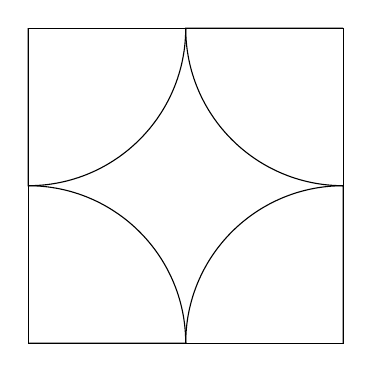
\begin{tikzpicture}
            \smallskip
            \draw (0,0) -- (0,4) -- (4,4) -- (4,0) -- (0,0);
            \draw (0,0) -- +(0:2cm) arc (0:90:2cm);
            \draw (0,4) -- +(270:2cm) arc (270:360:2cm);
            \draw (4,4) -- +(180:2cm) arc (180:270:2cm);
            \draw (4,0) -- +(90:2cm) arc (90:180:2cm);
        \end{tikzpicture}
    \\Answer:\fbox{$\frac{4-\pi}{4}$}}
    \item {Noah and Ben are playing a dice game. First, Noah rolls a twenty sided die with numbers from 1 to 20. If the result is 13 or higher, then he is allowed to roll two six-sided dice with numbers from 1 to 6, and sum them to determine how many points he gets. Ben opts to make the rules slightly more interesting. He will give Noah 10 extra points automatically whenever Noah rolls the six sided dice but Noah will only get to roll them if the result on the twenty sided die is 18 or higher instead of 13 or higher. How many fewer points can Noah expect to earn under the new system than under the old one? \textbf{NCC 2019 - E8} \\Answer: \fbox{0.25 or $\frac{1}{4}$}}
\end{enumerate}

\end{document}
